\begin{figure}[t]
    \centering
    % --- 第一个子图 (Claude) ---
    \begin{subfigure}[b]{0.99\columnwidth}
        \centering
        % width=\linewidth 让图片充满子图的宽度
        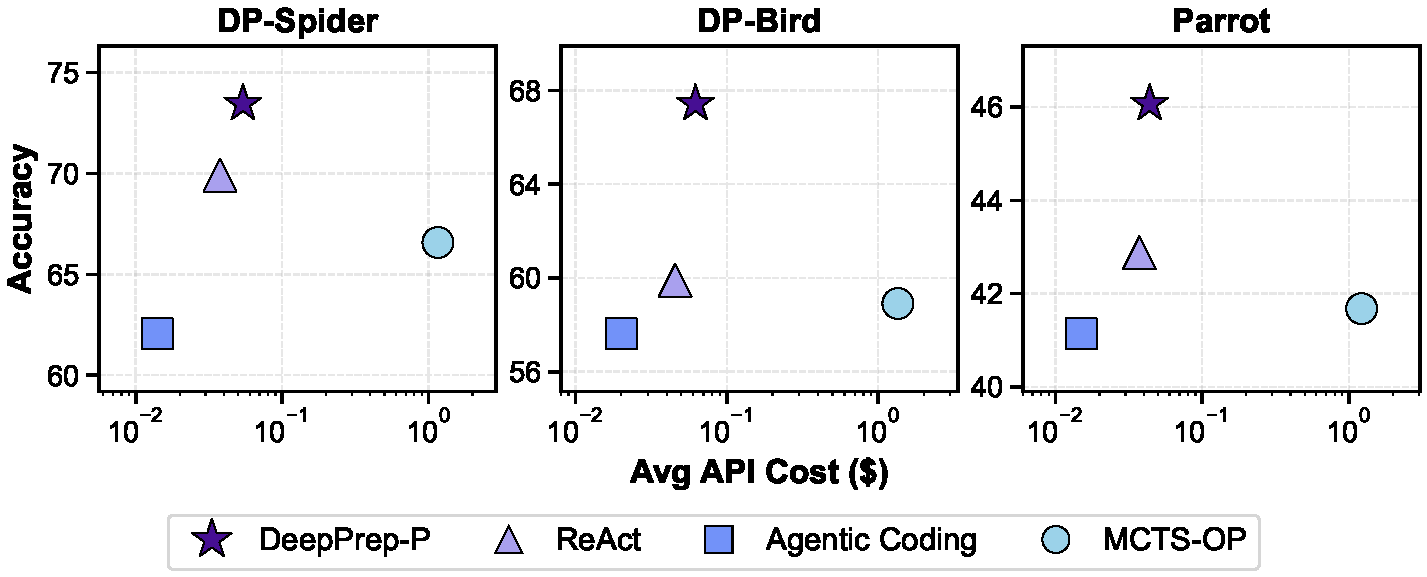
\includegraphics[width=\linewidth]{plots/plot/acc_cost_tradeoff_claude.pdf}
        \caption{Claude} % 这里写该子图对应的 LLM 名称
        \label{fig:acc_cost_tradeoff_claude}
    \end{subfigure}
    
    \vspace{1em} % 调整两个子图之间的垂直间距
    
    % --- 第二个子图 (R1) ---
    \begin{subfigure}[b]{0.99\columnwidth}
        \centering
        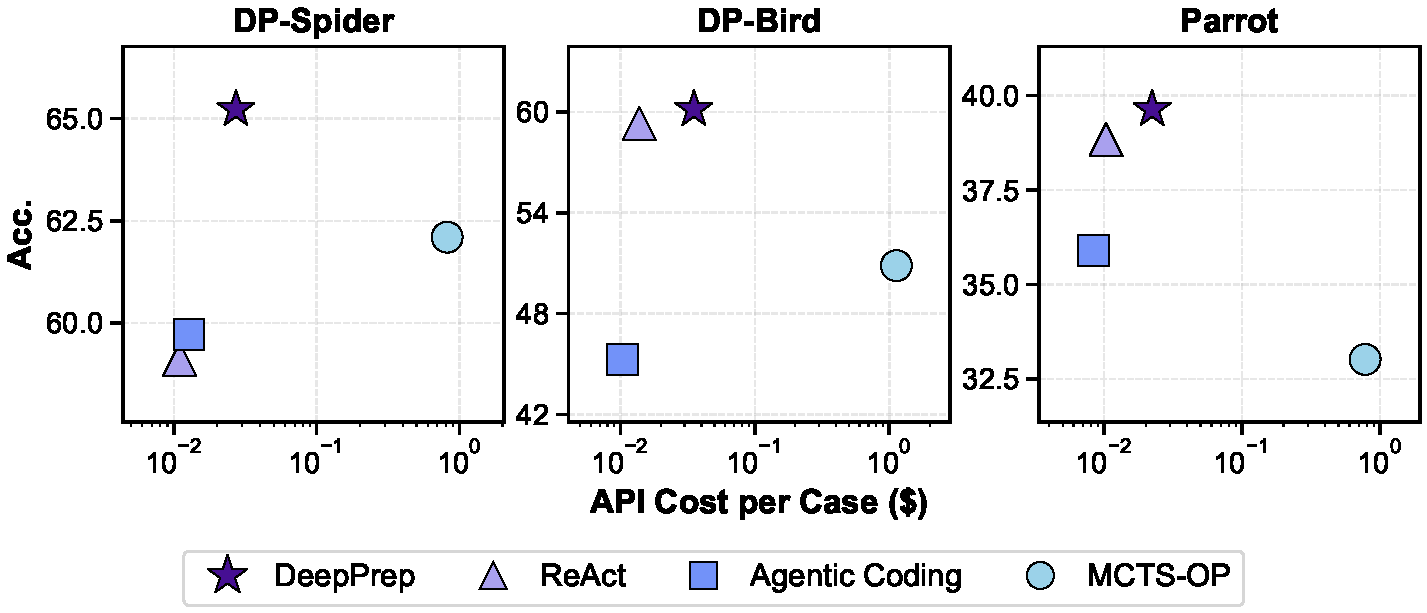
\includegraphics[width=\linewidth]{plots/plot/acc_cost_tradeoff_r1.pdf}
        \caption{R1} % 这里写该子图对应的 LLM 名称
        \label{fig:acc_cost_tradeoff_r1}
    \end{subfigure}
    
    \vspace{-0.5em} 
    % 总标题
    \caption{Trade-off between Accuracy and API cost. We compare the performance on (a) Claude and (b) R1.}
    \label{fig:acc_cost_tradeoff_combined}
    \vspace{-1em}
\end{figure}
